\chapter{Theoretical Motivation}\label{ch:theory}

The LHC is capable of producing proton-proton collisions with a center-of-mass energy of up to $\sqrt{s}=14~\mbox{TeV}$. Accounting for the composite nature of the proton, these collisions give access to phenomena with characteristic energies approximately up to the TeV scale, which couple in some fashion to quarks or gluons. To date, the Standard Model (SM) of Particle Physics has accurately described most phenomena observed in collider experiments up to this energy scale. A small number of observations, however, as well as a few technical and aesthetic concerns, reveal deficiencies in the theory. Numerous theories have been proposed to remedy the deficiencies, many of which make testable predictions for the LHC.

This chapter describes the theories underlying the LHC's exploration of physics at the TeV scale. The Standard Model physics is described first, followed by its known shortcomings and their possible consequences at the LHC. Emphasis is placed on theories predicting the production of several charged leptons, which are the subject of the searches described in chapters~\ref{ch:model-independent-trilepton-search} and \ref{ch:trilepton-resonance-search}.


\section{The Standard Model}\label{sec:standard-model}
The Standard Model of particle physics is a theoretical framework describing the dynamics and interactions of the known elementary particles under the electromagnetic, weak, and strong forces. The theory is a gauge theory describing a wide range of phenomena in the language of Quantum Field Theory. Particles are described as excitations of quantum fields, whose properties are defined by their representations under the Lorentz group and the gauge groups associated with the electroweak and strong forces. This section briefly introduces the Standard Model in the context of proton-proton collisions at the LHC.


\subsection{Gauge Theory}

%Force particles, or \emph{vector bosons}, have spin $s=1$, and obey Bose-Einstein statistics. These consist of twelve gauge bosons associated to the twelve generators of $G_{\mathrm{SM}}$. Matter particles, or \emph{fermions}, have $s=\frac12$, and obey Dirac statistics~\cite{spin-statistics}. The fermions of the Standard Model consist of quarks and leptons. Quarks are charged under the whole gauge group, experiencing both the strong force, which confines them into hadrons, and the electroweak force, responsible for radioactive decays and electromagnetic interactions. Leptons and neutrinos, on the other hand, are charged only under $\mathrm{SU}(2)_L\times U(1)_Y$, and experience only the electroweak force. Finally, the Standard Model contains a single scalar boson with $s=0$, called the Higgs boson.

A \emph{gauge theory} is a quantum field theory in which the Lagrangian is invariant under local transformations under a gauge group $G$~\cite{peskinschroeder}. To give a simple example, consider a single massless fermion field $\psi(x)$, with kinetic term,

\begin{equation}
	\mathcal{L} = i\overline{\psi}(x) \slashed{\partial} \psi(x),
\end{equation}
where $\slashed{\partial}\equiv \gamma^{\mu}\partial_{\mu}$ and $\gamma^{\mu}$ are the $\gamma$-matrices associated with the Lorentz group. To introduce a gauge group $G$, the Lagrangian is required to be invariant under local transformations under the action of $G$:
 \begin{align*}
 	\psi(x) &\rightarrow V(x) \psi(x), \\
 	V(x) &= e^{i\alpha(x)^a t^a} \\
 \end{align*}
 where $t^a$ are the generators of the Lie algebra of $G$, and $\alpha(x)_a$ are arbitrary continuous functions. The kinetic term in the Lagrangian, $i\overline{\psi}(x)\gamma^{\mu}\partial_{\mu}\psi(x)$, can be made invariant by promoting the simple derivate $\partial_{\mu}$ to a \emph{covariant derivative}, $D_{\mu}$, defined as:

\begin{equation}\label{eqn:covariant-derivative-qcd}
	D_{\mu} = \partial_{\mu} - i g t^a A^a_{\mu},
\end{equation}

where $g$ is a coupling constant associated with the gauge interaction and $A^a_{\mu}(x)$ are vector fields associated with the gauge bosons of $G$, which transform under the action of $G$ as:

\begin{equation}\label{eqn:gauge-field-transformation}
	A^a_{\mu}(x)t_a \rightarrow V(x) \left(A^a_{\mu}(x)t^a + \frac{i}{g} \partial_{\mu}\right) V^{\dagger}(x) \\
\end{equation}

For infinitesimal $\alpha(x)^a$, the transformations can be expressed as:
\begin{align}\label{eqn:gauge-field-transformation-infinitesimal}
	\psi(x)&\rightarrow (1 + i\alpha^a t^a + \mathcal{O}(\alpha^2))\psi(x) \\
	A^a_{\mu} &\rightarrow A_{\mu}^a + \frac{1}{g}\partial_{\mu}\alpha^a(x) + f^{abc}A^b_{\mu}\alpha^c + \mathcal{O}(\alpha^2),
\end{align}
where $f^{abc}$ are the structure constants of $G$, defined by
\begin{equation}
	[t^a,\ t^b] = if^{abc}t^c.
\end{equation}

Note that the structure constants are zero for Abelian gauge groups, such as $G=U(1)$. The Lagrangian for the gauge theory, including gauge-invariant terms involving $A^a_{\mu}(x)$ itself, is:

\begin{equation}\label{eqn:simple-gauge-lagrangian}
	\mathcal{L} = \overline{\psi}(x) (i\slashed{D}) \psi(x) - \frac{1}{4} (F^a_{\mu\nu})^2,
\end{equation}

where $F_{\mu\nu}^a=\partial_{\mu}A^a_{\nu}(x) - \partial_{\nu} A^a_{\mu}(x) + g f^{abc}A_{\mu}^b A_{\nu}^c$ is the field strength tensor of $A^a_{\mu}(x)$. 

The interactions of the fields $\psi(x)$ and $A^a_{\mu}(x)$ are manifest in the Lagrangian. In this example, the interaction of $\psi$ with $A^a$ is described by the interaction term
\begin{equation}
	\mathcal{L}_{\mathrm{int}} = \overline{\psi} \gamma^{\mu}A^a_{\mu}t^a \psi.
\end{equation}

For non-Abelian gauge groups with nonzero structure constants $f^{abc}$, the square of the field strength tensor also yields cubic and quartic self-interaction terms amongst the $A^a_{\mu}(x)$.



\subsection{Particle Content}
The Standard Model is a gauge theory with gauge group $G_{\mathrm{SM}}=SU(3)_c\times SU(2)_L \times U(1)_Y$, roughly corresponding to the strong, weak, and electromagnetic forces, respectively. The theory contains a fermion field for every observed matter particle. The fermions can be grouped into three generations, each containing an up-type quark with charge $\pm\frac23$, a down-type quark with charge $\pm\frac13$, a lepton with charge $\pm1$, and a neutrino with charge $0$. The generations are identical except for the particles' masses. The fermions and their transformation properties under the Standard Model gauge group are listed in table~\ref{table:standard-model-particles}. The quarks are charged under all three gauge groups, and thus interact via the strong, weak, and electromagnetic forces. The leptons, on the other hand, are only charged under $\mathrm{SU}(2)_L\times \mathrm{U}(1)_Y$, and hence interact via the weak and electromagnetic forces, but not the strong force. 

The bosonic content of the Standard Model consists of the spin-0 Higgs boson, plus a spin-1 boson for each generator of $\mathrm{SU}(3)_c\times SU(2)_L \times U(1)_Y$, yielding eight gluons for $\mathrm{SU}(3)_c$ and four electroweak gauge bosons for $\mathrm{SU}(2)_L\times U(1)_Y$. 

% Consider doing TJ's strategy of describing the basic principles of constructing the SM, a la Iliopolous. 

\begin{table}[htbp]
	\centering
	\begin{tabular}{cccccc}
		 & $Q_L=\left(\begin{array}{c} u_L \\ d_L \end{array}\right)$ & $u_R$ & $d_R$ & $E_L=\left(\begin{array}{c} \nu_L \\ e_L \end{array}\right) $ & $e_R$ \\
		$\mathrm{SU}(3)_c$ & $\mathbf{3}$ &  $\mathbf{3}$ & $\mathbf{3}$ & $\mathbf{1}$ & $\mathbf{1}$ \\
		$\mathrm{SU}(2)_L$ & $\mathbf{2}$ & $\mathbf{1}$ & $\mathbf{1}$ & $\mathbf{2}$ & $\mathbf{1}$ \\
		$\mathrm{U}(1)_Y$ & $\frac16$ & $\frac23$ & $-\frac13$ & $-\frac12$ & $-1$ \\
	\end{tabular}
	\caption{Matter particles (fermions) in a single generation of the Standard Model, their representations under $\mathrm{SU}(3)_c$ and $\mathrm{SU}(2)_L$, and their charges under $\mathrm{U}(1)_Y$. The left- and right-handed fermions are distinguished by the subscripts $L$ and $R$.}
	\label{table:standard-model-particles}
\end{table}

%\begin{table}
%	\centering
%	\begin{tabular}{|c|c|c|}
%		\hline
%		$e$ & $u$ & $d$ \\
%		\hline
%		$0.510998928 \pm 0.000000011$ & $2.3^{+0.7}_{-0.5}$ & $4.8^{+0.5}_{-0.3}$ \\
%		\hline
%		\hline
%		$\mu$ & $c$ & $s$ \\
%		\hline
%		$105.6583715 \pm 0.0000035$ & $1275\pm25$ & $95\pm5$ \\
%		\hline
%		\hline
%		$\tau$ & $t$ & $b$ \\
%		\hline
%		$1776.82 ± 0.16$ & $173.21\times10^3\pm 510 \pm 710$ & $4.18\times10^3 \pm 30$ \\
%		\hline
%	\end{tabular}
%	\caption{List of Standard Model fermions and their masses. Neutrinos are omitted from the table; though the observation of neutrino oscillations indicate that they have nonzero mass, only the squares of the mass differences between the three neutrino mass eigenstates, $\Delta m_{ij}^2$, have been measured.}
%	\label{table:fermion-masses}
%\end{table}


\subsection{Strong Sector}
% Introductory paragraph: Quarks are charged under SU(3), giving three colors of quark times six quark flavors. The strong force confines five of the six into color-neutral hadrons. Write down some examples... like, the strange mesons, for example. 

% Important point 1: confinement. Write down the running of the coupling, and show that it diverges (or at least appears to). Renders perturbation theory ineffective. 

% Important point 2: asymptotic freedom. The flip side of the gauge coupling running is that the coupling decreases with energy, so the theory is perturbative at high energies. 

% Long lifetimes: Quarkonia with low bound state energies have to decay via off-diagonal CKM matrix elements, so charm and bottom mesons often have long lifetimes.

% Very short lifetime: the top quark decays too fast to hadronize. 


The strong sector of the Standard Model is a non-abelian $\mathrm{SU}(3)_c$ gauge theory, describing the interactions of quarks under the strong force. The theory, called \emph{quantum chromodynamics} (QCD), contains the six observed quarks, called the up, down, charm, strange, top, and bottom quarks, as well as eight massless force carriers called gluons. 

QCD describes drastically different phenomena at high and low energies. At low energies, the most tangible consequence of the strong interaction, perhaps, is that most of the matter in the universe is composed of protons and neutrons, not individual quarks. Indeed, free quarks have never observed in nature, except for the short-lived top quark; rather, quarks are always confined into hadrons, bound states of quarks that are neutral under the strong interaction. On the other hand, in the high energy limit, the strength of the interaction becomes small, and quarks and gluons behave as nearly free particles.

This behavior, called \emph{asymptotic freedom}, was described in 1973 by Wilczek and Gross, and independently Politzer~\cite{Gross:1973id,Politzer:1973fx}. Under the renormalization group, the strong coupling constant, $\alpha_s = \frac{g_s}{4\pi}$, changes with the energy scale of the interaction, $Q$. To one-loop order in $\alpha_s$, the running of $\alpha_s$ is given by:

\begin{equation}
\alpha_s(Q) = \frac{\alpha_s(M)}{1 + (b_0 \alpha_s/2\pi)\log(Q/M)},
\end{equation}

where $b_0=11-\frac{2}{3}n_f$ for $n_f$ fermion fields, and $M$ is an arbitrary energy scale at which the strong coupling constant $\alpha_s(M)$ has been measured. With $n_f=6$, corresponding to the six quark flavors, $\frac{\mathrm{d}\alpha_s(Q)}{\mathrm{d}Q}<0$; hence the coupling decreases as $Q$ increases. At high energies, $Q\gtrsim \SI{1}{\giga\electronvolt}$, quarks interact weakly, and perturbative calculations are reliable. On the other hand, as $Q$ decreases, $\alpha_s(Q)$ increases. The one-loop expression diverges at
\begin{equation}
Q=M\exp\left(\frac{8\pi^2}{b_0g^2}\right) \equiv \Lambda_{\mathrm{QCD}}.
\end{equation}

Note that this calculation is perturbative in $\alpha_s$, and becomes unreliable once $\alpha_s$ becomes large in the vicinity of the divergence. Experimental measurements indicate $\Lambda_{\mathrm{QCD}}\approx \SI{200}{\mega\electronvolt}$~\cite{Campbell:1998gr}. 


\subsubsection{Proton-Proton Collisions}
The proton-proton collisions at the LHC involve several characteristic energy scales, such as the scale of the interaction between constituents of the protons, $Q^2$, or the masses of the various particles participating in the interactions. Calculations rely on QCD factorization~\cite{Collins:2004tz}: hard, perturbative processes, namely the hard scattering between constituents of the protons, factorize from soft, non-perturbative processes, such as the description of the behavior of those constituents within the proton. 

The composite nature of the colliding protons is described by the \emph{parton model}, developed in the context of deep inelastic scattering experiments and generalized to hadron-hadron collisions~\cite{Bjorken:1969ja,feynmanparton,Drell:1970yt}. Protons are described as collections of pointlike particles, or partons, bound together by their interactions. In the center-of-mass reference frame, the incoming protons are highly boosted. The time scale of the collision is very short due to Lorentz contraction, while the internal interactions among partons are time dilated and do not influence the hard scattering. The essence of factorization is that while the interactions of the remaining partons can affect the eventual outcome of the collision, they do not interfere quantum mechanically with the hard scattering, and hence their effect can be factorized at the level of probabilities, rather than amplitudes.

Over the short duration of the collision, the colliding parton can be assigned a definite fraction $x$ of the total proton momentum. The partons are characterized by universal \emph{parton distribution functions} (PDFs), $f_{a/A}(x_a,\,\mu_F^2)$, which describe the probability that parton $a$ within hadron $A$ carries a fraction $x_a$ of the total hadron momentum. The factorization scale, $\mu_F$, roughly represents the scale dividing long- and short-distance processes, and is usually chosen to be near the scale of the hard scattering interaction, $\mu_F\sim Q^2$~\cite{Campbell:2006jf}. Cross sections for a given interaction are calculated by summing over the relevant partons and integrating over the PDFs:

\begin{equation}
	\sigma_{AB\rightarrow X} = \sum_{a\in A,\,b\in B}\int \mathrm{d}x_a\, \mathrm{d}x_b\, f_{a/A}(x_a,\,\mu_F^2) f_{b/B}(x_b,\,\mu_F^2) \hat{\sigma}_{ab\rightarrow X},
\end{equation}

where $a$ and $b$ represent partons within protons $A$ and $B$ with momentum fractions $x_a$ and $x_b$, respectively, and $\hat{\sigma}_{ab\rightarrow X}$ is the hard scattering cross section for those partons. The PDFs are determined from fits to existing data; the dependence on $x$ must be determined from the data, while the dependence on the factorization scale can be derived from the DGLAP equations~\cite{Gribov:1972ri,Dokshitzer:1977sg,Altarelli:1977zs}. An example is shown in figure~\ref{fig:theory-pdf-example}. Note that this calculation depends on the choice of unphysical scales, $\mu_F$ and also the scale of renormalization used in the calculation of $\hat{\sigma}$, effectively due to the truncation of the calculation at finite order in the perturbative expansion. Theoretical systematic uncertainties are assigned by varying these scales up and down, e.g. by factors of 2. 

\begin{figure}[htbp]
	\centering
	\hfill
	\subfloat[] {
		\resizebox{0.4\textwidth}{!}{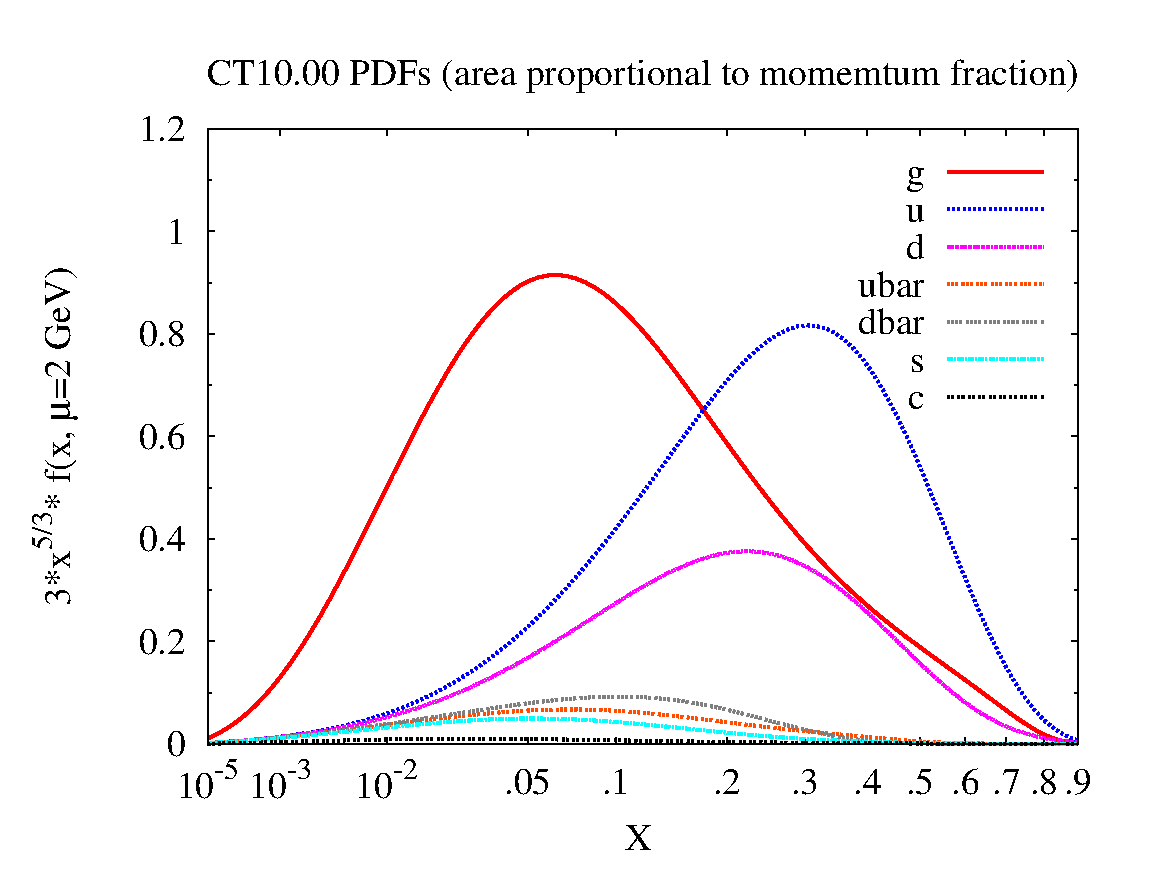
\includegraphics{figures/theory/pdf-ct10Q2a}}
	}
	\hfill
	\subfloat[] {
		\resizebox{0.4\textwidth}{!}{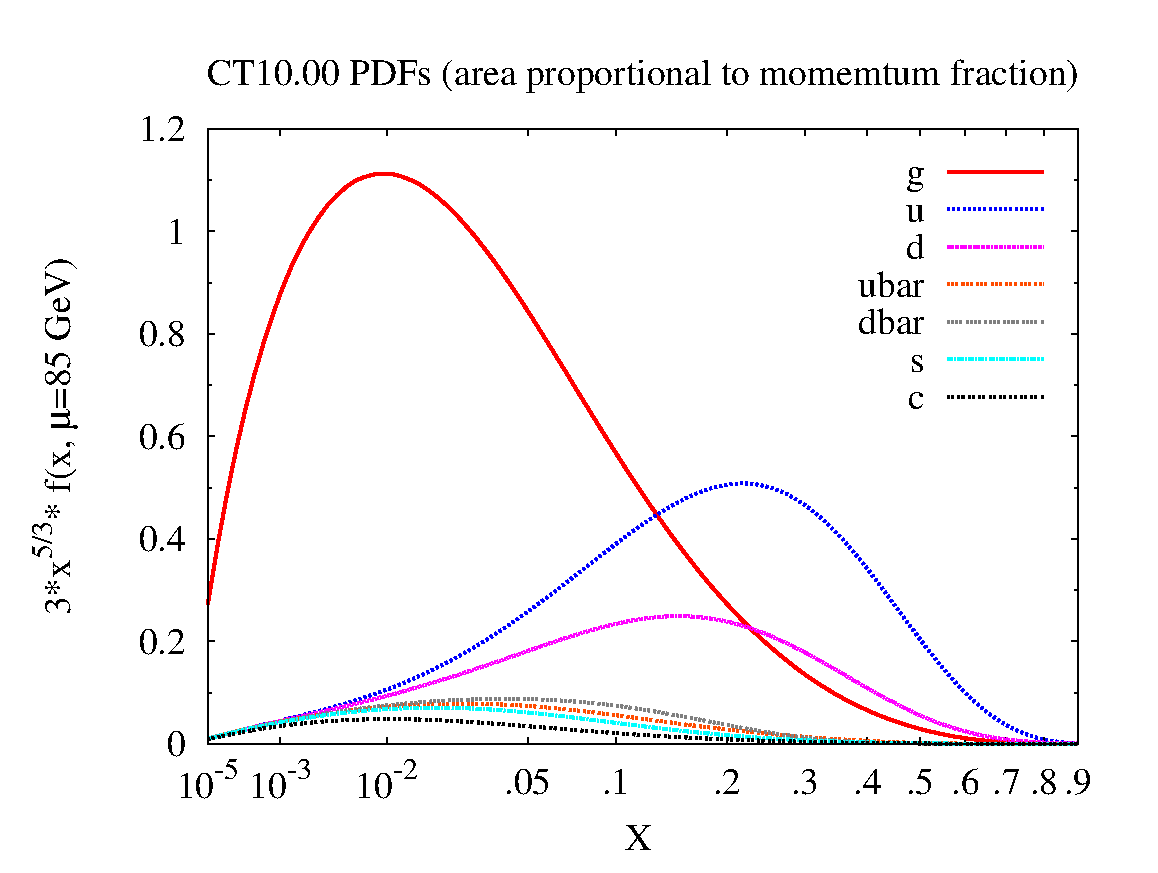
\includegraphics{figures/theory/pdf-ct10Q85a}}
	}
	\hfill
	\caption{Example parton distribution functions at $\mu=\SI{2}{\giga\electronvolt}$ and $\mu=\SI{85}{\giga\electronvolt}$, from the CT10 PDF set~\cite{ct10}.}
	\label{fig:theory-pdf-example}
\end{figure}

\subsubsection{Jets}
A typical proton-proton collision will typically produce several colored partons, from the hard scattering interaction itself or from QCD radiation from initial or final state partons. Free quarks are not observed in nature due to confinement, and hence the colored partons are not directly observed. Rather, the partons transform into a collection of color-neutral hadrons, which are observed as clusters of particles called \emph{jets}. Quarks and gluons emerging from the collision radiate additional gluons, while the gluons split into quark-antiquark pairs. The splittings, which are dominated by the emission of soft and collinear radiation, continue until the local momentum scales reach $\mathcal{O}(\SI{1}{\giga\electronvolt})$, at which point QCD becomes strongly interacting and confines the partons into hadrons. 

The process of jet formation can be modeled using a \emph{parton shower} algorithm, which describes probabilistically the addition of soft or collinear partons to the event beyond the hard scattering process~\cite{Buckley:2011ms}. Hadronization is a non-perturbative process, and hence cannot be computed from QCD. It is instead described by phenomenological models, such as the Lund string model~\cite{Andersson:1983ia} or the cluster model~\cite{Webber:1983if}, which incorporate many free parameters to tune to data. 


\subsection{Electroweak Sector}
The electroweak sector is a unified description of electromagnetism and weak decays as a gauge theory with gauge group $\mathrm{SU}(2)_L\times U(1)_Y$. The theory models a number of phenomena, including:
\begin{itemize}
	\item The weak decays of heavy quarks and leptons.
	\item The nonzero masses of the weak gauge bosons, quarks, and charged leptons.
	\item Flavor violation in weak decays involving charged currents.
	\item Violation of $C$-, $P$-, and $CP$-symmetry observed in certain decay processes~\cite{Wu:1957my,Christenson:1964fg,Collaboration:1999jz,AlaviHarati:1999xp}.
\end{itemize}

The underlying theory of the electroweak sector is rather more complicated than the strong sector. $C$ violation is manifest in the construction of the theory: the gauge couplings are \emph{chiral}, with the left- and right-handed components of fermions belonging to different representations of $\mathrm{SU}(2)$. Such a symmetry forbids mass terms for the fermions and gauge bosons, in clear conflict with observations. To accommodate fermion and gauge boson masses without abandoning the symmetry, a scalar Higgs field is added with a quartic potential arranged such that the ground state spontaneously breaks the $\mathrm{SU}(2)_L$ symmetry. The resulting theory contains a large number of free parameters: two gauge couplings $g$ and $g'$, two constants in the quartic Higgs potential, nine Yukawa couplings between the fermions and the Higgs field, and three mixing angles and one phase in the CKM matrix. 

%The Lagrangian can be broken into two pieces, $\mathcal{L} = \mathcal{L}_{\mathrm{sym}} + \mathcal{L}_{\mathrm{Higgs}}$, where the first piece contains terms with only gauge bosons and fermion fields and conserves $\mathrm{SU}(2)_L$ symmetry, and the second piece contains terms with Higgs fields and spontaneously breaks $\mathrm{SU}(2)_L$ symmetry. 

In the this and the following sections, $W^{a\mu}$ represents the three $\mathrm{SU}(2)_L$ gauge fields, $B^{\mu}$ the $\mathrm{U}(1)_Y$ gauge field, and $\phi$ the Higgs scalar field, which is a complex $\mathrm{SU}(2)_L$ doublet. Assigning the left-handed components of fermions to the doublet $\mathrm{SU}(2)_L$ representation and the right-handed components to the singlet presentation, the Standard Model quarks are denoted by $Q_L^i\equiv \left(\begin{array}{c} u^i_L \\ d^i_L \end{array}\right)$, $u_R^i$, and $d_R^i$, where $i=1,2,3$ indicates the generation. Similarly, the leptons are denoted by $E_L^i\equiv \left(\begin{array}{c} \nu_L^i \\ e_L^i \end{array}\right)$ and $e_R^i$. There is no corresponding right-handed neutrino in the theory. 

\subsubsection{The Higgs Mechanism}
Much of the phenomenology of the electroweak sector can be derived starting from the observation that the $W^{\pm}$ and $Z^0$ bosons have masses of nearly $\SI{100}{\giga\electronvolt}$, as heavy as entire krypton or molybdenum atoms. Straightfowardly adding explicit gauge boson masses in the Lagrangian, e.g. $m_W^2 (W_{\mu}^a)^2$, fails immediately  due to the requirement of gauge invariance. It is easy to see that such terms in not invariant under equation~\ref{eqn:gauge-field-transformation-infinitesimal}.

% , inspired by developments in superconductivity in the early 1960s~\cite{Nambu:1960tm + anderson?},
The solution to this quandary is that the ground state of the theory need not exhibit the same symmetries as the underlying Lagrangian. This phenomenon, known as spontaneous symmetry breaking, underlies the Higgs mechanism~\cite{Higgs:1964pj,Englert:1964et,Guralnik:1964eu}, and is realized in the model of Glashow, Salam, and Weinberg~\cite{Glashow:1961tr,Weinberg:1967tq,Salam:1968rm}. 

The model introduces an $\mathrm{SU}(2)$ doublet of scalar fields, $\phi$, with Lagrangian,


\begin{equation}\label{eqn:higg-lagrangian}
	\begin{multlined}
		\mathcal{L}_{\mathrm{Higgs}} = |D_{\mu}\phi|^2 - V(\phi^{\dagger}\phi),
	\end{multlined}
\end{equation}

where the potential energy term given by:
\begin{equation}\label{eqn:higgs-potential}
	V(\phi^{\dagger}\phi) = \frac12 \mu^2 \phi^{\dagger}\phi + \frac14 \lambda (\phi^{\dagger}\phi)^2.
\end{equation}


The quartic potential induces electroweak symmetry breaking if the quadratic coefficient is negative, i.e. $\mu^2<0$. The potential is then minimized for a nonzero value of $\phi$. Using the $\mathrm{SU}(2)_L$ symmetry, we can take vacuum expectation value of $\phi$ to be:

\begin{equation}
	\langle \phi \rangle = \frac{1}{\sqrt{2}} \left(\begin{array}{c} 0 \\ v \end{array}\right).
\end{equation}
 
Solving for $v$,

\begin{align}
	0 = \frac{\mathrm{d}V}{\mathrm{d}v} &= -\frac12\mu^2 v + \frac14\lambda v^3 \\
	v &= \frac{2\mu^2}{\lambda}.
\end{align}

Expanding the Higgs field about its expectation value, $\phi$ can be written:

\begin{equation}
	\phi = U \frac{1}{\sqrt{2}} \left(\begin{array}{c} 0 \\ v+H \end{array}\right),
\end{equation}

where $U$ is a local $\mathrm{SU}(2)$ gauge transformation that can be set to $\mathbf{1}$ by choice of gauge. 

The masses and interactions of various particles are described by expanding the Higgs field about $\langle \phi \rangle$ and identifying the relevant physical states. For the Higgs field itself, the potential energy terms are:

\begin{equation}
	\Delta \mathcal{L} = -\frac12 m_H^2 H^2 - \sqrt{\frac{\lambda}{2}} m_H H^3 - \frac14 \lambda H^4,
\end{equation}

 where $m_H=\sqrt{2}\mu$. The theory thus predicts a massive scalar boson with cubic and quartic self interactions.


\subsubsection{Gauge Bosons}
The mass terms for the gauge bosons arise from the covariant derivative terms in equation~\ref{eqn:higg-lagrangian}. Expanding the covariant derivates, the relevant mass terms are:

\begin{equation}
	\Delta\mathcal{L} = \frac{1}{8} v^2 \left( g^2 (W^1_{\mu}W^{1\mu} + W^2_{\mu}W^{2\mu}) + (g'B_{\mu} - gW^3_{\mu})^2 \right).
\end{equation}

The physical states are the gauge- and mass-eigenstates,
\begin{align}
	W^{\pm}_{\mu} &= \frac{W^1 \mp iW^2}{\sqrt{2}} \label{eqn:weak-diag-W} \\
	Z^0_{\mu} &= -\sin\theta_w B_{\mu} + \cos\theta_w W_{\mu}^3 \label{eqn:weak-diag-Z}\\
	A_{\mu} &= \cos\theta_w B_{\mu} + \sin\theta_w W_{\mu}^3\label{eqn:weak-diag-A},
\end{align}

where $\tan\theta_w = \frac{g'}{g}$. The corresponding masses are:
\begin{align}
	m_{W^{\pm}} &= \frac{gv}{2} \\
	m_{Z^0} &= \frac{gv}{2\cos\theta_w} \\
	m_{A} &= 0.
\end{align}

The theory thus predicts a nontrivial relationship between the masses of the gauge bosons, $m_{W^{\pm}}$ and $m_{Z^0}$, and the gauge coupling constants $g$ and $g'$.

\subsubsection{Fermion Masses}\label{sec:standard-model-fermion-masses}
The fermion masses arise from the Yukawa coupling terms between the fermions and the Higgs field,
\begin{equation}\label{eqn:lagrangian-yukawa-couplings}
	-\Delta \mathcal{L} = - \left(\lambda_d^{ij} \overline{Q}_L^i \cdot \phi d_R^j - \lambda_u^{ij} \epsilon^{ab}\overline{Q}^i_{La} u_R^j + \mathrm{h.c.}\right) - \left(\lambda_l^{ij} \overline{E}^i_L \cdot \phi e_R^j + \mathrm{h.c.}\right).
\end{equation}
 
 The $\lambda_{u,d,l}^{ij}$ are complex matrices of coupling constants. These are, in general, not symmetric or Hermitian, and to identify the physical mass eigenstates, the matrices must be diagonalized. The Yukawa matrices can be decomposed using the singular value decomposition as:

\begin{equation}
	\lambda_u = U_u D_u W_u^{\dagger},\ \lambda_d = U_d D_d W_d^{\dagger},\ \lambda_l = U_l D_l W_l^{\dagger},
\end{equation}
 
where $U_{u,d,l}$ and $W_{u,d,l}$ are unitary matrices, and $D_{u,d,l}$ are diagonal, non-negative matrices. Making a change of variables,

\begin{align}\label{eqn:yukawa-diagonalization}
	u_L^i\rightarrow U_{u}^{ij}u_L^j&,\ d_L^i\rightarrow U_d^{ij}d_L^j, \\
	u_R^i\rightarrow W_{u}^{ij}u_R^j&,\ d_R^i\rightarrow W_d^{ij}d_R^j, \\
	e_L^i\rightarrow U_l^{ij}e_L^j&,\ \nu_L^i\rightarrow U_l^{ij}\nu_L^j, \\
	e_R^i\rightarrow W_l^{ij}e_R^j&,
\end{align}

the off-diagonal Yukawa couplings vanish as intended, while the kinetic terms remain invariant. The masses of the fermions are:

\begin{equation}
	m_u^i = \frac{1}{\sqrt{2}} D_u^{ii}v,\ m_d^i = \frac{1}{\sqrt{2}} D_d^{ii}v,\ m_l^i = \frac{1}{\sqrt{2}} D_l^{ii}v,\ m_{\nu}^i = 0.
\end{equation}


\subsubsection{Weak Interactions of Fermions}
The Lagrangian describing the interactions of fermions and gauge bosons is:

\begin{equation}\label{eqn:electroweak-lagrangian}
	\mathcal{L}_{\mathrm{sym}} =  -\frac{1}{4} \sum_{i=1}^3  \overline{E}_L (i\slashed{D}) E_L + \overline{e}_R(i\slashed{D})e_R + \overline{Q}_L(i\slashed{D})Q_L + \overline{u}_R(i\slashed{D})u_R+\overline{d}_R(i\slashed{D})d_R,
\end{equation}

where, similarly to equation~\ref{eqn:covariant-derivative-qcd}, the covariant derivative $D_{\mu}$ is given by:

\begin{align}\label{eqn:covariant-derivative-ew}
	D_{\mu} &= \partial_{\mu} - i g \tau^a W^{a}_{\mu} - i g' Y B_{\mu}, \\
\end{align}

where the $\tau^a$ are operators corresponding to the action of a given generator of the $\mathrm{SU}(2)_L$ Lie algebra, and $Y$ is an operator corresponding to the action of the generator of $\mathrm{U}(1)_Y$, which simply returns the hypercharge. For the left-handed doublets in the fundamental representation of $\mathrm{SU}(2)_L$, the $\tau^a$ can be taken to be the Pauli matrices, $\tau^a=\frac12 \sigma^a$. For right-handed singlets in the trivial representation of $\mathrm{SU}(2)_L$, the $\tau^a$ are zero. In other words, the right-handed fermions do not interact with the $W^{a\mu}$. 

In terms of the physical gauge bosons, given in equations~\ref{eqn:weak-diag-W}--\ref{eqn:weak-diag-A}, 
\begin{align}
	D_{\mu} &= \partial_{\mu} - i \frac{g}{\sqrt{2}}\left(W_{\mu}^+ \tau^+ + W_{\mu}^- \tau^-\right) - i\frac{g}{\cos\theta_w} Z_{\mu}\left(\tau^3 - \sin^2\theta_w Q\right) - i e A_{\mu} Q,
\end{align}

where $e=\frac{gg'}{\sqrt{g^2+g'^2}}$, $\tau^{\pm}=\left(\tau^1 \pm i \tau^2\right)$, and $Q=\tau^3+Y$. 

The fermion couplings to the gauge bosons are complicated by the fact that the mass eigenstates do not necessarily coincide with the gauge eigenstates, due to the off-diagonal Yukawa couplings in section~\ref{sec:standard-model-fermion-masses}. The diagonalization procedure alters the couplings of the quarks to the $W^{\pm}$ bosons. The quark-$W^{\pm}$ couplings can be written in terms of the current $J^{\mu\pm}=\sum_{i} \frac1{\sqrt{2}}\left(\overline{u}_L^i\gamma^{\mu}d_L^i\right)$ as:

\begin{equation}
	\Delta\mathcal{L} = g (W^+_{\mu}J^{\mu+}_W + W^{-}_{\mu}J^{\mu -}_{W})
\end{equation}

Under the transformation in equation~\ref{eqn:yukawa-diagonalization}, $J^{\mu\pm}\rightarrow \sum_{ij}\frac{1}{\sqrt{2}} \overline{u}_L^i \gamma^{\mu} V^{ij} d_L^j$, where $V^{ij}$ is a $3\times 3$ unitary matrix known as the \emph{Cabibbo-Kobayashi-Maskawa} (CKM) matrix, $V = U_{u}^{\dagger} U_d$. The non-zero off-diagonal elements of $V$ imply that weak decays mix the three generations of quarks; quark flavor is not conserved in weak decays, as is readily observed in hadron decays, e.g. $K^{\pm}\rightarrow \pi^{\pm}+\pi^0$. Further, $V$ contains one nontrivial complex phase, allowing for $CP$ violation in weak decays. 

Note that the lepton sector does not contain an analogous mixing matrix for weak decays, due to the presence of only a single Yukawa matrix $\lambda^{ij}_l$. Hence lepton flavor and $CP$ are conserved in leptonic weak decays.

\subsubsection{Trilepton Production}
In proton-proton collisions at the LHC, the production of three or more charged leptons proceeds through at least two electroweak gauge bosons, which can be real or virtual, or a Higgs boson. The branching fractions of $W^{\pm}$ and $Z^0$ bosons to leptons are shown in table~\ref{table:theory-WZ-BR}. Leptons can be produced in several ways (neglecting leptons due to interactions with the detector for the moment):

\begin{itemize}
	\item Weak gauge bosons decaying directly to leptons: $W^{\pm}\rightarrow \ell^{\pm}\nu_{\ell}$ or $Z^0\rightarrow \ell^{\pm}\ell^{\mp}$.
	\item Drell-Yan production: $pp\rightarrow Z/\gamma^{*}\rightarrow\ell^{\pm}\ell^{\mp}$. 
	\item Higgs bosons decaying directly to leptons: $H\rightarrow \ell^{\pm}\ell^{\mp}$, where $\ell=e$, $\mu$, or $\tau$. In practice, this is significant only for $\tau$ leptons, as the Higgs couplings to electrons and muons are very small.
	\item Higgs bosons decaying indirectly to leptons: $H\rightarrow W^{\pm}W^{\mp*}$ or $H\rightarrow ZZ^{*}$, where the weak gauge bosons decay leptonically.
	\item Leptonically or semileptonically decaying hadrons: $J/\psi\rightarrow \mu^+\mu^-$ or $K^+\rightarrow \pi^0 e^+ \nu_{e}$. 
\end{itemize}

\begin{table}[htbp]
	\centering
	\hfill
	\subfloat[ $W$] {
		\begin{tabular}{cc}
			\ \\
			Decay & Branching Fraction \\
			\hline
			$e\nu$	&	$10.71\pm 0.16\ [\%]$ \\
			$\mu\nu$	&	$10.63\pm 0.15\ [\%]$ \\
			$\tau\nu$	&	$11.38\pm 0.21\ [\%]$ \\
			Hadrons 	&	$67.41\pm 0.27\ [\%]$ \\ 
			\ 
		\end{tabular}
	}
	\hfill
	\subfloat[ $Z$] {
		\begin{tabular}{cc}
			Decay & Branching Fraction \\
			\hline
			$e^+e^-$		&	$3.363 \pm 0.004\ [\%]$ \\
			$\mu^+\mu^-$	&	$3.366 \pm 0.007\ [\%]$ \\
			$\tau^+\tau^-$	&	$3.370 \pm 0.008\ [\%]$ \\
			Invisible		&	$20.00 \pm 0.06\ [\%]$ \\
			Hadrons			&	$69.91 \pm 0.06\ [\%]$ \\
			$4\ell$ ($\ell=e,\mu$)	&	$(3.20\pm0.28)\times10^{-6}$~\cite{TheATLASCollaboration:2014db} \\
		\end{tabular}
	}
	\hfill
	\caption{Branching fractions of $W^{\pm}$ and $Z^0$ bosons to leptons and other final states~\cite{pdg}.}
	\label{table:theory-WZ-BR}
\end{table}

The dominant source of events containing at least three charged leptons is diboson production, $q\overline{q}'\rightarrow W^{\pm}Z^0$ or $q\overline{q}'\rightarrow Z^0Z^0$, where the bosons decay leptonically. Production of two top quarks with a gauge bosons, $t\overline{t}+V\rightarrow W^{\pm}W^{\mp}b\overline{b}+V$ where $V=W^{\pm}$ or $Z^0$, contributes to a lesser extent. The production of three gauge bosons, $VVV^{(*)}$, is taken into account, but is generally negligible. The estimation of Standard Model trilepton production is discussed in more detail in section~\ref{sec:prompt-backgrounds}. 



\section{Beyond the Standard Model}\label{sec:bsm}
Though quite successful as a description of most observed phenomena in particle physics, the Standard Model is deficient in several ways. Several observations indicate that the particle content is incomplete; additionally, the theory has a few unsatisfying constructional aspects which, while not technically inconsistent, suggest that there remains underlying physics to be discovered. Many theories have been proposed to solve these issues, and confronting these theories is a major goal of the ATLAS experiment. This section describes the motivations for searching for physics beyond the Standard Model (BSM), and lists several of the leading BSM theories which can be confronted at the LHC.

\subsection{Shortcomings of the Standard Model}\label{sec:bsm-unexplained-phenomena}

Several observations over the last few decades, largely from astrophysics and cosmology, are not described by the Standard Model. These include:

\begin{itemize}
	\item \textbf{Neutrino mass}: Due to the lack of right-handed neutrinos and left-handed antineutrinos, neutrinos are massless in the Standard Model. However, observation of neutrino flavor oscillations indicate that at least two of the three neutrinos have nonzero mass. The phenomenon of oscillation was first observed by the Homestake solar electron neutrino detector~\cite{Cleveland:1998nv}, in the form of a deficit of electron neutrinos detected from the sun. Later experiments observed oscillation among other types of neutrinos and antineutrinos, from a variety of sources including the sun, nuclear reactors, cosmic rays interacting with the atmosphere, and particle accelerators~\cite{pdg}. The data imply that the three neutrino mass eigenstates have different masses, with differences given by:
	\begin{align}\label{eqn:neutrino-mass-differences}
		|\Delta m_{21}^2| &\cong 7.5\times 10^{-5}~\mbox{eV}^2 \\
		|\Delta m_{31}^2| &\cong 2.5\times 10^{-3}~\mbox{eV}^2.
	\end{align}
	These relations hold only if at least two of the neutrino masses are nonzero. On the other hand, $\beta$-decay experiments and cosmological observations indicate an upper bound on the neutrino mass scale of order $m_{v_i} \lesssim \mathcal{O}(0.1-\SI{1}{\electronvolt})$~\cite{Aseev:2011ia, Abazajian:2011ck, Ade:2013zuv}.

	\item \textbf{Dark matter}: Astrophysical observations suggest the existence of a large amount of non-Standard Model matter which interacts only gravitationally with baryonic matter. The earliest tension with known physics comes from galactic rotation curves, the distribution of rotational velocities of stars about the galactic center as a function of radius~\cite{1980ApJ_238_471R}. The rotational velocities $v(r)$ can be compared with the expectation from the observed matter distribution, $\tilde{v}(r)=\sqrt{\frac{M(r)}{r}}$, where $M(r)$ is the observed mass at radius less than $r$. At large distances from the galactic center, the observed rotation curve behaves like $v(r)\sim$constant, while the expected rotation curves behaves like $v(r)\sim \frac{1}{\sqrt{r}}$. 

	At present, the leading explanation for the discrepancy is the presence of a large amount of gravitationally interacting, non-luminous matter in galaxies, known as \emph{dark matter}. The hypothesis is supported by cosmological observations: measurements of anisotropies in the cosmic microwave background (CMB) are sensitive to the relative amounts of baryonic matter (which interacts with photons), dark matter (which does not), and dark energy. A recent combination of CMB measurements gives the following values~\cite{Ade:1530686}:
	\begin{align}
		\Omega_{c}h^2 &= 0.1198 \pm 0.0026, \\
		\Omega_{b}h^2 &= 0.02207 \pm 0.00027, \\
		\Omega_{\Lambda} &= 0.685^{+0.017}_{-0.016}, \\
	\end{align}
	where $\Omega_{c}$ and $\Omega_{b}$ are the density parameters for cold dark matter and baryonic matter, respectively, $h$ is the Hubble constant, and $\Omega_{\Lambda}$ is the cosmological constant. 

	Many candidates have been proposed as the constituents of dark matter, such as primordial black holes, sterile neutrinos, axions, and weakly interacting massive particles (WIMPs). WIMPs are a particularly interesting candidate for LHC phenomenology: in the so-called ``freeze-out'' model of dark matter evolution, $\Omega_c$ is fixed when dark matter falls out of thermal equilibrium with conventional matter. $\Omega_c\sim0.1$ is achieved with $m_{\chi}\sim \mathcal{O}(100~\mbox{GeV})$ and couplings of order $g_X\sim\mathcal{O}(0.1-1)$; such a particle could be produced and detected at the LHC. 

	\item \textbf{Matter-Antimatter Asymmetry}: The observable universe is made up of matter and photons, with very little antimatter. Astrophysical observations measure the ratio of baryons (minus antibaryons) to photons,
	\begin{equation}\label{eqn:baryon-photon-ratio}
		\eta \equiv \frac{n_B - n_{\overline{B}}}{n_{\gamma}}, 
	\end{equation}
	to be in the range $5.7\times 10^{-10} \leq \eta \leq 6.7\times 10^{-10}$ at $95\%$ confidence level~\cite{pdg-bbn}. However, assuming symmetrical initial conditions and conservation of baryon number, the Big Bang would produce baryons and antibaryons in equal number\footnote{Asymmetric initial conditions are disfavored due to inflation, which would dilute any initial asymmetry~\cite{cline}.}. Due to inefficient annihilation after freeze-out, the present abundances would be $\frac{n_B}{n_{\gamma}} = \frac{n_{\overline{B}}}{n_{\gamma}} \approx 10^{-20}$~\cite{cline}. The generation of a large baryon-antibaryon asymmetry is known as the \emph{baryogenesis} problem.

	%Three conditions are necessary for baryogenesis, known as the Sakharov conditions~\cite{sakharov}: baryon number violation, $C$- and $CP$-symmetry violation, and interactions out of thermal equilibrium (i.e. the interaction rate must be slower than the expansion rate of the universe). In principle, the Standard Model possibly satisfies all three conditions: baryon number is violated by electroweak sphaelerons~\cite{thooft}, $C$ and $CP$ violation is observed in hadron oscillations and decays~\cite{Kindirect, Kdirect,B,D}, and thermal equilibrium may be lost if the electroweak phase transition is sufficiently first-order~\cite{???}. However, baryogenesis of sufficient magnitude has not been demonstrated, in particular due to insufficient $CP$-violation. 

	\item \textbf{Gravity}: Gravity is not described by the Standard Model. 

\end{itemize}

\subsection{Theoretical Issues}\label{sec:bsm-theoretical-deficiencies}
Besides not describing the phenomena listed above, the Standard Model has a number of theoretical issues related to its parameters and structure.

\begin{itemize}
	\item \textbf{Hierarchy problem}: The hierarchy problem refers to the large discrepancy between the electroweak scale, $\mathcal{O}(\SI{e2}{\giga\electronvolt})$, and the Planck scale, $\mathcal{O}(\SI{e19}{\giga\electronvolt})$. Due to fermion and gauge boson loops like those shown in figure~\ref{fig:higgs-mass-feyman-diagrams}, the Higgs boson mass receives quantum corrections proportional to $\Lambda^2$, where $\Lambda$ is the scale up to which the theory is valid. For example, due to a fermion $f$ with Yukawa coupling $\lambda_f$, the physical Higgs mass at one loop order is:

	\begin{equation}\label{eqn:higgs-mass-divergence}
		m_{H,\mathrm{phys}}^2 \approx m_{H}^2 -\frac{|\lambda_f|^2}{8\pi^2} \Lambda^2,
	\end{equation}

	where $m_{H}^2$ is the bare Higgs mass parameter in the Lagrangian. In practice, the contribution from the top quark, with $\lambda_t\sim1$, dominates this expression. If $\Lambda$ is near the Planck scale, $\Lambda\sim\SI{e19}{\giga\electronvolt}$, then with $m_H(\mathrm{phys})=\SI{125.7}{\giga\electronvolt}$, the bare Higgs mass and $\Delta m_H^2$ must cancel to some 30 orders of magnitude, an unsavory coincidence referred to as \emph{fine tuning}. Turning the problem on its head, if nature is not finely tuned, then $\Lambda$ should be not too far above the electroweak scale, $\Lambda \lesssim \SI{10}{\tera\electronvolt}$. The physics responsible for such a cutoff scale could be accessible at the LHC. 

	\begin{figure}[htbp]
		\centering
		\hfill
		\subfloat[] {
			\resizebox{0.4\textwidth}{!}{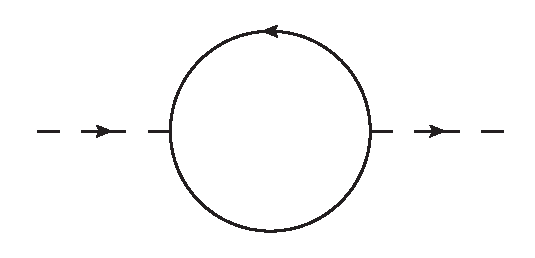
\includegraphics{figures/fd/Higgs_1loop_fermion}}
		}
		\hfill
		\subfloat[] {
			\resizebox{0.4\textwidth}{!}{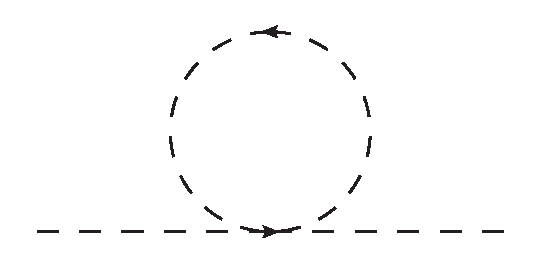
\includegraphics{figures/fd/Higgs_1loop_boson}}
		}
		\hfill
		\caption{One-loop Feynman diagrams involving fermions (left) and bosons (right) leading to the quadratic divergence of the Higgs mass.}
		\label{fig:higgs-mass-feyman-diagrams}
	\end{figure}
	

	\item \textbf{Strong $CP$ problem}: The strong sector of the Standard Model potentially contains a $CP$-violating term, 
	\begin{equation}
		\mathcal{L}_{\Theta}=\theta_{\mathrm{QCD}} \frac{\alpha_s}{8\pi}G^{\mu \nu a} \tilde{G}^{a}_{\mu\nu},
	\end{equation}
	where $-\pi\leq\theta_{\mathrm{QCD}}\leq\pi$ is the effective $\Theta$ parameter after diagonalizing the quark mass matrix, $G^{a}_{\mu\nu}=\partial_{\mu}\mathcal{A}_{\mu}^{a}-\partial_{\nu}\mathcal{A}_{\mu}^{a} - g_s f^{abc}\mathcal{A}_{\mu}^{b} \mathcal{A}_{\nu}^{c}$ is the gluon field strength tensor, and $\tilde{G}^a_{\mu\nu}=\epsilon_{\mu\nu\alpha\beta}G^{\alpha\beta a}$ is its dual~\cite{pdg-axions}. However, this term is severely constrained by measurements of the neutron dipole moment~\cite{PhysRevLett.97.131801}, with a limit of $|\theta_{\mathrm{QCD}}|\lesssim 10^{-10}$. 

	Axions are a leading candidate for the resolution of the strong $CP$ problem~\cite{Peccei:400569}. These are typically very weakly coupled, and would not be observable at the LHC.

	\item \textbf{Free parameters}: The Standard Model contains 19 free parameters. In terms of measured quantities, these are the 6 quark masses $m_{q_i}$, 3 lepton masses $m_{l_i}$, 3 CKM mixing angles $\theta_{ij}$ and 1 CKM phase $\delta$, 3 gauge couplings $g_i$, the QCD vacuum angle $\theta_{\mathrm{QCD}}$, the Higgs field vacuum expectation value $v$, and the Higgs mass, $m_H$. These parameters are measured; their values are not predicted by the theory. It remains unknown why the Yukawa couplings range over six orders of magnitude, for example, nor why the fermions fall into three identical generations. 


	\item \textbf{Gauge Unification}: The origin of the Standard Model gauge group, $G_{SM}=SU(3)_c\times SU(2)_L \times U(1)_Y$, is not understood. Remarkably, the Standard Model fermion content can be described as a $\mathbf{5}^{*}\oplus \mathbf{10}$ representation of $\mathrm{SU}(5)$, the smallest simple group containing $G_{SM}$, with all of the Standard Model quantum numbers correctly predicted. Unfortunately, simply augmenting the gauge group to $\mathrm{SU}(5)$ leads to an unacceptable rate of proton decay, but deriving $G_{SM}$ from a larger, ``unified'' gauge group remains a topic of active investigation.  
\end{itemize}

\subsection{Theories of BSM Physics}\label{sec:bsm-theories}
A large number of theories have been developed to address the problems in the previous section, many of which yield testable predictions for the LHC. This section describes three examples of such theories: supersymmetry, extra fermions beyond the three Standard Model generations, and the neutrino seesaw mechanism. These theories are capable of producing three or more charged leptons in $pp$ collisions through the production and decay of heavy new particles, and can thus be confronted against the analyses described in chapters~\ref{ch:model-independent-trilepton-search} and \ref{ch:trilepton-resonance-search}.

\subsubsection{Supersymmetry}
The hierarchy problem described above motivates the consideration of additional symmetries. Consider again the Higgs mass quadratic divergence (equation~\ref{eqn:higgs-mass-divergence}). The divergence could be avoided by introducing scalar partners to the fermions to counteract the divergence, due to the relative (-) sign between scalar and fermion loops in figure~\ref{fig:higgs-mass-feyman-diagrams}. Cancelling the divergence at all orders suggests the introduction of an extra symmetry to the Standard Model. 

The forms that such a symmetry could take are quite restricted. In 1967, Coleman and Mandula demonstrated that, under a small set of physically assumptions, the symmetry algebra of the $S$-matrix must be isomorphic to a direct product of the Poincar\'{e} group and an internal symmetry group (i.e. whose generators commute with those of the Poincar\'{e} group). This \emph{no-go} theorem appeared to establish that it is impossible to ``[combine] space-time and internal symmetries in any but a trivial way.'' However, a loophole was found in 1975, formalized in the theorem of Haag, Lopuszanski, and Sohnius: the Poincar\'{e} group can be extended nontrivially in the context of graded Lie algebras, allowing the symmetry generators to be commuting or anticommuting~\cite{Haag1975257}. These so-called ``supersymmetries'', first proposed in by Wess and Zumino~\cite{Wess197439}, transform bosons to fermions and vice-versa, and combine nontrivially with the Poincar\'{e} group in that the anticommutator of two supersymmetry generators is a spacetime translation. 

By itself, supersymmetry predicts a partner for every Standard Model particle with identical mass and quantum numbers, except that the spin differs by 1/2. The symmetry is assumed to be spontaneously broken at some high mass scale, giving additional mass to the superpartners to account for the fact that superpartners have not yet been observed. The minimal implementation, called the \emph{minimal supersymmetric Standard Model} (MSSM), contains 178 free parameters, although simplifying assumptions are almost always used to reduce this enormous parameter space to manageable size.

Supersymmetry addresses a number of the shortcomings of the standard model described above. First, it provides a boson-fermion symmetry to cancel the quadratic divergence in the Higgs mass. Second, the superpartners are typically assigned an extra quantum number, $R$-parity, under with the SM particles are neutral, in order to stabilize the proton; this extra symmetry has the consequence of making the lightest supersymmetric particle (LSP) stable, providing a dark matter candidate. Third, the supersymmetry breaking sector contains numerous CP-violating parameters, which could provide the necessary CP violation to explain the matter-antimatter asymmetry in the universe. Finally, the superpartners modify the running of the three gauge couplings such that they approach similar values in the UV, supporting the notion of gauge unification. 

Trilepton events are a useful tool in MSSM searches. A common scenario is that the heavy supersymmetric particles decay back to Standard Model particles plus an LSP, often producing three or more leptons in the decay chains. Figure~\ref{fig:theory-susy-trilepton-example} shows an example involving the production of charginos and neutralinos, the superpartners of the $W^{\pm}$, $Z^0$, and $H$ bosons. ATLAS has performed several dedicated searches for such scenarios~\cite{TheATLASCollaboration:2014cs,Aad:2014ia,TheATLASCollaboration:2014hq}, which are not discussed in this dissertation. 

\begin{figure}[htbp]
	\centering
	\resizebox{0.4\textwidth}{!}{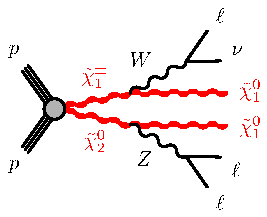
\includegraphics{figures/fd/C1N2-lllvN1N1-WZ}}
	\caption{Feynman diagram showing the production of a chargino, $\tilde{\chi}_1^{\pm}$, and a neutralino, $\tilde{\chi}^0_2$, decaying to two neutralino LSPs, $\tilde{\chi}^0_1$, plus three leptons and a neutrino. The chargino/neutralino subscript indicates mass ordering, with $1$ being the lightest.}
	\label{fig:theory-susy-trilepton-example}
\end{figure}



\subsubsection{Extra Generations of Matter}\label{sec:theory-bsm-vlf}
Given that the origin of the three generations of fermions is not understood, an obvious question is whether additional generations might exist. A review of extra fermions can be found at~\cite{Frampton:1999kr}. A fourth chiral generation, i.e. another copy of the three known generations, is strongly constrained, though not completely excluded~\cite{Buchkremer:2012gb,Djouadi:2012dm,Chanowitz:2013hk,Banerjee:2014gy}. The number of neutrinos coupling to the $Z$ boson with $m_{\nu}<\frac12 m_Z$ can be determined from the invisible width of the $Z$, giving $N_{\nu}= 2.9840 \pm 0.0084$. Further, additional chiral fermions coupling to the Higgs boson would significantly alter its production rate and decay patterns. The production cross section for $gg\rightarrow H$, in particular, increases by roughly a factor of 9. 

Additional non-chiral, or \emph{vector-like}, fermions are less constrained. Such fermions are defined as having identical left- and right-handed interactions under the Standard Model gauge group, particularly under $\mathrm{SU}(2)_L$. Consequently, explicit mass terms, $m\overline{\psi}\psi$, are not forbidden by gauge invariance, and the fermions need not couple to the Higgs field to acquire mass. The impact on Higgs production and decay, as well as precision electroweak observables, are small. Further, the pattern of extra vector-like fermions is less restricted compared to chiral generations, where a spectacular cancellation between the fields of each generation is needed to avoid chiral anomalies. 

Vector-like fermions are a feature of many model of BSM physics. Additional quarks are present in some models addressing the hierarchy problem, such as the little Higgs model~\cite{Arkani-Hamed:557546} or composite Higgs models~\cite{Kaplan:148688}. Vector-like leptons can appear alongside quarks in $\mathrm{SU}(5)$ multiplets~\cite{Martin:2012dx}, and are predicted in models explaining the fermion mass hierarchy~\cite{Falkowski:2014hs}, composite Higgs models, models with warped extra dimensions~\cite{Redi:2013ib,Contino:1005586}, and the type~III neutrino seesaw mechanism, discussed in section~\ref{sec:theory-bsm-seesaw}. 

In order to render the vector-like fermions unstable, mixing terms involving the Standard Model fermions can be introduced. This enables decays to a $W^{\pm}$, $Z^0$, or $H$ boson, plus a Standard Model quark or lepton. Three or more leptons can be produced if the bosons decay leptonically. In the case of vector-like leptons, the three leptons can also be produced resonantly, allowing the use of a trilepton mass constraint. The collider phenomology of vector-like leptons is discussed in more detail in section~\ref{sec:resonance-signal-models}.



\subsubsection{Neutrino Seesaw}\label{sec:theory-bsm-seesaw}
Due to the lack of right-handed neutrinos in the Standard Model, neutrinos are exactly massless. A neutrino mass term, $m_{\nu} \overline{\nu}_L \nu_L^c$ violates $\mathrm{SU}(2)_L$ gauge invariance. An effective mass term arising perturbatively, e.g. $\frac{Y_{ij}}{v}\phi\phi L_i L_j$, would be a good candidate to explain the small size of neutrino masses due to suppression from the mass scale $v$, but turns out to be forbidden as well due to the accidental conservation of lepton number, $L$, and also baryon minus lepton number, $B-L$~\cite{RevModPhys.75.345}. 

If neutrinos are their own antiparticle, i.e. are Majorana fermions rather than Dirac fermions, a leading candidate to explain the small but nonzero neutrino masses is the \emph{neutrino seesaw mechanism}~\cite{Mohapatra:1980yp,GellMann:1980vs,Yanagida:1980xy}. The Standard Model is augmented with heavy, sterile neutrinos, $N_i$, which have both Majorana masses and Yukawa interactions with the Standard Model neutrinos:
\begin{equation}
	\mathcal{L}_N = \frac12 M_{N_{ij}} \overline{N}^c_i N_j + Y_{ij}^{\nu} \overline{L}_{i} \tilde{\phi} N_{j} + \mathrm{h.c.}
\end{equation}

where $L_i = \left(\begin{array}{c}\nu_i \\ \ell_i \end{array}\right)$. The resulting mass matrix takes the form:

\begin{equation}
	M_{\nu} = \left(\begin{array}{cc} 0 & Y^{\nu} \frac{v}{\sqrt{2}} \\ (Y^{\nu})^T \frac{v}{\sqrt{2}} & M_N \end{array}\right)
\end{equation}
in the basis $\left(\begin{array}{c} \nu_{i} \\ N_j \end{array} \right)$. If $M_N \gg v$, then diagonalizing the mass matrix gives three eigenstates will light masses, $m_{\nu_{L_i}} \sim  \frac{Yv^2}{M_N}$. With $v=246~\mbox{GeV}$, a light neutrino mass of $m_{\nu}=0.1~\mbox{eV}$ gives a heavy neutrino mass of:
\begin{equation}
	M_N \sim Y \times 10^{15}~\mbox{GeV}.
\end{equation}

Hence Yukawa couplings of order 1 predict heavy, sterile neutrinos around the GUT scale, while smaller couplings predict a proportionally smaller mass scale. New mass scales accessible at the LHC can be achieved with more complicated models, such as the inverse seesaw model~\cite{inverse seesaw}, which introduce more mass scales and high powers of the suppression factors.

At tree level, there are three possible implementations of the seesaw mechanism: 
\begin{itemize}
	\item \textbf{Type I}: The simplest realization of the seesaw mechanism, at least two sterile neutrinos $N_i$ are introduced as described above. This scenario is not likely to be testable at the LHC, due to the combination of small Yukawa couplings and large sterile neutrino masses required for $\mathcal{O}(0.1~\mbox{eV})$ neutrino masses. 

	\item \textbf{Type II}: The seesaw mechanism is generated by an $\mathrm{SU}(2)_L$ triplet of scalars, $\Delta$, with hypercharge $Y=2$. This allows the construction of the following Yukawa term:
	\begin{equation}
		-\mathcal{L} = Y^{\Delta}_{ij} L_{i}^T C \sigma_2 \Delta L_{j} + \mathrm{h.c.},
	\end{equation}
	where $i$ ranges over the three lepton flavors.  Assuming diagonal Yukawa couplings for simplicity, the neutral component of the triplet, $\Delta^0$, acquires a vacuum expectation value,
	\begin{equation}
		v_{\Delta} = \frac{\mu v^2}{\sqrt{2} m_{\Delta}^2},
	\end{equation}
	where $m_{\Delta}$ is the mass term for $\Delta$, $\mu\sim m_{\Delta}$ is a coefficient of the cubic Higgs-$\Delta$ interaction with mass dimension 1, and $v$ is the Standard Model Higgs vacuum expectation value. The light neutrinos acquire mass:
	\begin{equation}
		m_{\nu_{i}} \sim Y^{\Delta}_{i} v_{\Delta}=Y^{\Delta}_{i} \frac{\mu v^2}{\sqrt{2} m_{\Delta}^2}.
	\end{equation}

	The triplet of scalars can potentially be produced via gauge interactions at the LHC, if their masses are below the TeV scale. The new particle content consists of $\Delta^0$, $\Delta^{\pm}$, and $\Delta^{\pm\pm}$. Same-sign dilepton final states have been used to search for the doubly charged scalar~\cite{TheATLASCollaboration:2015gu}, and $\Delta^{\pm\pm}\Delta^{\mp\mp}$ pair production is used as a benchmark model for the model-independent trilepton search presented in chapter~\ref{ch:model-independent-trilepton-search}. 


	\item \textbf{Type III}: The seesaw mechanism is generated by at least two $\mathrm{SU}(2)_L$ triplets of fermions with hypercharge $Y=0$,
	\begin{equation}
		\Sigma = \Sigma^a \sigma^a = \left(\begin{array}{cc} \Sigma^0/\sqrt{2} & \Sigma^+ \\ \Sigma^- & -\Sigma^0/\sqrt{2} \end{array}\right). 
	\end{equation}
	The Lagrangian is:
	\begin{equation}
		\mathcal{L}_{\Sigma} = Tr[i\overline{\Sigma}\slashed{D}\Sigma] - \frac12 Tr[\overline{\Sigma}M_{\Sigma}\Sigma^c+\overline{\Sigma^c}M_{\Sigma}^{*}\Sigma] - \tilde{\phi}^{\dagger}\overline{\Sigma}\sqrt{2}Y_{\Sigma}L - \overline{L}\sqrt{s}Y_{\Sigma}^{\dagger}\Sigma \tilde{\phi},
	\end{equation}
	where $L=(\nu,l)^T$, $\phi=(\phi^+, \phi^0)^T$, $\tilde{\phi}=i\sigma_2\phi^{*}$, and $\Sigma^c=C\overline{\Sigma}^T$. Summation over lepton flavor is implicit. The neutral fermion $\Sigma^0$ generates the seesaw mechanism in much the same way as in the type I implementation, giving neutrino masses:
	\begin{equation}
		m_{\nu} = -v^2 Y_{\Sigma}^T \cdot M_{\Sigma}^{-1} \cdot Y_{\Sigma}
	\end{equation}
	
	Like the scalar triplet, the heavy fermion triplet can also be produced at detectable rates at the LHC via gauge interactions. The collider phenomenology of the fermions, which are vector-like, is described in more detail in section~\ref{sec:resonance-signal-models}. 
\end{itemize}

\printbibliography